\clearpage
\section{Annex}
\subsection{Source files}
\subsubsection{Client}
\inputminted[
    fontsize=\small,
    linenos]{erlang}{src/client.erl}

\clearpage

\subsubsection{Server}
\inputminted[
    fontsize=\small,
    linenos]{erlang}{src/server.erl}

\clearpage

\subsubsection{Server2}
\inputminted[
    fontsize=\small,
    linenos]{erlang}{src/server2.erl}
    
\clearpage
\subsection{Screenshots}

\subsubsection{Server1 and clients (local)}

\begin{figure}[ht]
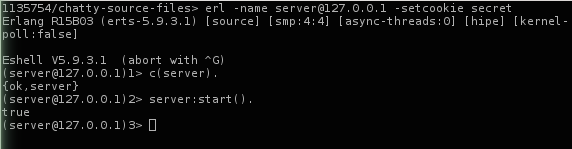
\includegraphics[scale=0.7]{server1}
\caption{Server1 running in pc \textit{a5s113pc43}}
\end{figure}

\begin{figure}[ht]
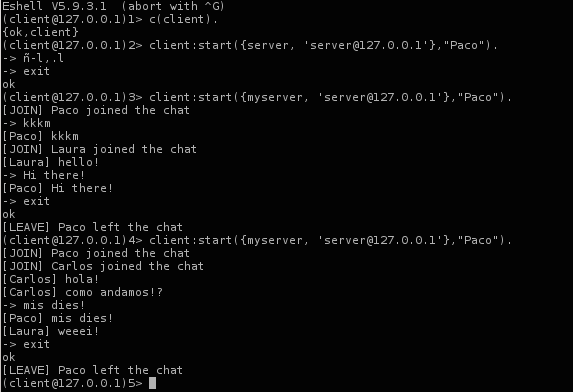
\includegraphics[scale=0.7]{clientPaco}
\caption{Client1 in Server1}
\end{figure}

\begin{figure}[ht]
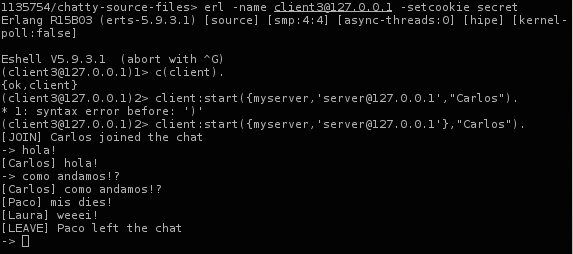
\includegraphics[scale=0.7]{clientCarlos}
\caption{Client2 in Server1}
\end{figure}

\begin{figure}[ht]
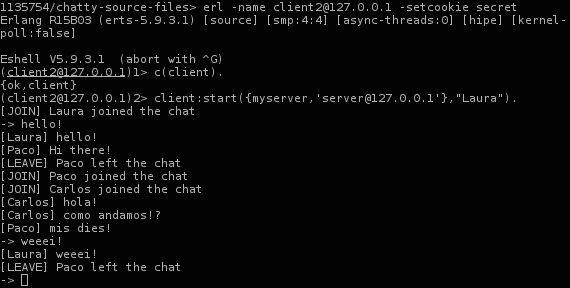
\includegraphics[scale=0.7]{clientLaura}
\caption{Client3 in Server1}
\end{figure}

% ------------- Experiments with separated PC's
\clearpage
\subsubsection{Server2 and clients (distributed)}
\begin{figure}[ht]
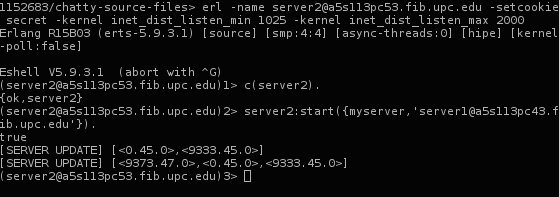
\includegraphics[scale=0.7]{server2Enrique-Remote}
\caption{Server2 running in pc \textit{a5s113pc53}}
\end{figure}

\begin{figure}[ht]
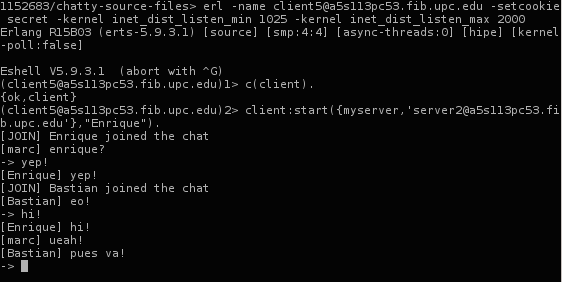
\includegraphics[scale=0.7]{clientEnrique-Remote}
\caption{Client running in pc \textit{a5s113pc53}}
\end{figure}

\begin{figure}[ht]
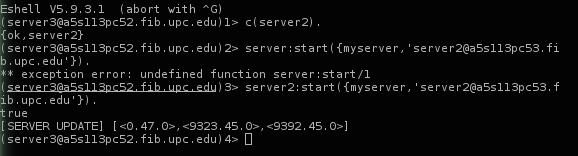
\includegraphics[scale=0.7]{server2Bastian-Remote}
\caption{Server2 running in pc \textit{a5s113pc52}}
\end{figure}

\begin{figure}[ht]
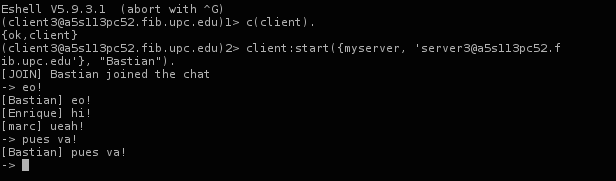
\includegraphics[scale=0.7]{clientBastian-Remote}
\caption{Client running in pc \textit{a5s113pc52}}
\end{figure}

\begin{figure}[ht]
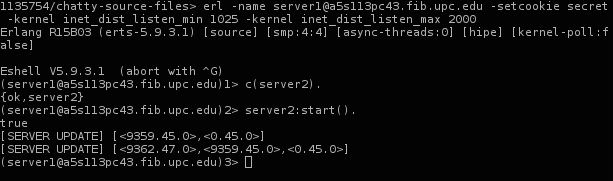
\includegraphics[scale=0.7]{server2Marc-Remote}
\caption{Server2 running in pc \textit{a5s113pc43}}
\end{figure}

\begin{figure}[ht]
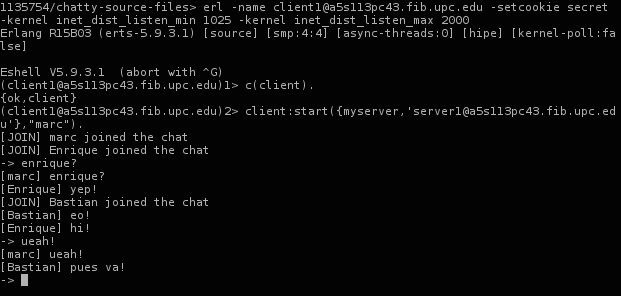
\includegraphics[scale=0.7]{clientMarc-Remote}
\caption{Client running in pc \textit{a5s113pc43}}
\end{figure}